\documentclass{standalone}
\usepackage{pgfplots}
\usetikzlibrary{intersections}
\usepgfplotslibrary{fillbetween}
\pgfplotsset{compat=1.7}

\begin{document}
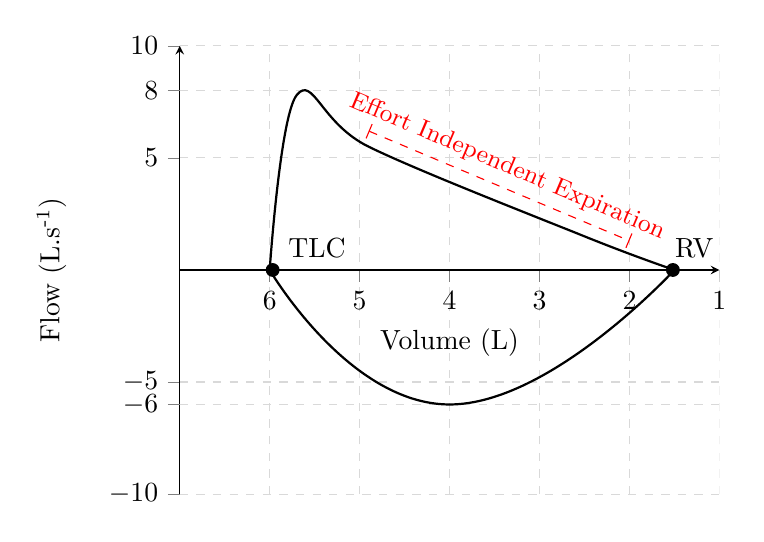
\begin{tikzpicture}

\begin{axis}[
     axis lines=middle,
     grid = major,
     grid style={dashed, gray!30},
	ylabel near ticks,
	xlabel near ticks,
	ymin = -10,
	ymax = 10,
	xmin = 0,
	xmax =6,
	xlabel near ticks,
	ylabel near ticks,
	extra y ticks = {-6, 8},
	xticklabels={,,6,5,4,3,2,1},
        xlabel=Volume (L),
        ylabel=Flow (L.s\textsuperscript{-1}),
        tick align=outside]

\draw[black, thick] plot[smooth, tension=0.9] coordinates { (axis cs: 5.5, 0) (axis cs: 3,-6) (axis cs: 1,0)};
\draw[black, thick] plot[smooth, tension=0.6] coordinates { (axis cs: 1,0) (axis cs: 1.3, 7.8)  (axis cs: 2.1, 5.5) (axis cs: 4.5, 1.5)  (axis cs: 5.5,0)};
\node[circle,fill=black,inner sep=0pt,minimum size=5pt] at (axis cs: 5.4,0) {};
\node[black] at (axis cs: 5.4,1) {RV};
\node[circle,fill=black,inner sep=0pt,minimum size=5pt] at (axis cs: 0.95,0) {};
\node[black] at (axis cs: 1.1,1) {TLC};


\tikzset{anchor=west}
\draw[red, dashed, |-|] (axis cs: 2.1, 6.2) -- node[red, above, rotate=-23, font=\small]{Effort Independent Expiration} (axis cs: 5, 1.3);

\end{axis}

\end{tikzpicture} 
\end{document}